\documentclass[11pt]{article}
\usepackage[margin=1in]{geometry}     % See geometry.pdf to learn the layout options. There are lots.
\geometry{letterpaper}                   % ... or a4paper or a5paper or ...
%\geometry{landscape}                % Activate for for rotated page geometry
%\usepackage[parfill]{parskip}    % Activate to begin paragraphs with an empty line rather than an indent

% \VignetteIndexEntry{An R Package for determining differential abundance in high throughput sequencing experiments}

\usepackage{graphicx}
\usepackage{amssymb}
\usepackage{epstopdf}
\usepackage{wrapfig}
\usepackage[margin=1in,font=small,labelfont=bf,
               labelsep=colon]{caption}

\DeclareGraphicsRule{.tif}{png}{.png}{`convert #1 `dirname #1`/`basename #1 .tif`.png}



\title{CoDaSeq: Compositional Data Analysis tools for high throughput sequencing}
\author{Greg Gloor}
\date{\today}                                           % Activate to display a given date or no date

\usepackage{Sweave}
\begin{document}

\maketitle
\tableofcontents
%\listoffigures
%\listoftables
\section{What is CoDaSeq?}
CoDaSeq is a suite of tools for the exploratory and analytical analysis of high throughput DNA sequencing data in a compositional data analysis (CoDa) framework. Many high throughput sequencing approaches generate similar data: reads are mapped to features in each sample, these features are normalized, then exploratory data analysis and statistical analysis is performed. CoDaSeq provides a simple consistent framework for data analysis that encompasses many different experimental designs by modelling the data as centre-log ratio transformed values rather than normalized counts or as proportions or relative abundances.

CoDaSeq provides a number of functions for the exploration and display of these data and builds upon a number of other R packages for compositional data analysis.

\section{Introduction}

\section{Installation}
Download and install the most current of CoDaSeq. It has been tested with version R version 3, but should run on version 2.12 onward. ALDEx2 will make use of the BiocParallel package if possible, otherwise, ALDEx2 will run in serial mode.

\section{Exploratory data analysis example of a 16S rRNA gene sequencing experiment using the `ak\_op' example data}

The ak\_op dataset is a small subset of the HMP oral microbiome dataset samples, with 15 samples from the attached keratinized gingiva and 15 samples from the external tooth plaque. These data are used as an example because they are extraordinarily sparse and represent a worst-case scenario for dealing with sparsity. The user is encouraged to try different filtering parameters to explore how filtering by abundance or sparsity affects the results.

First we load the library and the data and filter it by abundance.

\begin{Schunk}
\begin{Sinput}
> library(CoDaSeq)
> library(zCompositions)
> data(ak_op)
> data(hmpgenera)
> # the first function is to subset the dataselex
> f <- codaSeq.filter(ak_op, min.reads=1000, min.prop=0.01, max.prop=1,
+     min.occurrence=0.25, samples.by.row=FALSE)
> 
> # this should leave 167 OTUs and 30 samples
\end{Sinput}
\end{Schunk}

CoDaSeq contains several different ways to filter datasets.

\begin{description}
\item[min.reads] Sample-based filter to keep only samples with a minimum number of reads
\item[min.prop] OTU-based filter to keep only OTUs that have a proportional abundance greater than the cutoff in any sample. Values range from 0-1. Use 0 to keep all OTUs that have at least one read in any sample.
\item[max.prop] OTU-based filter to keep only OTUS that have a proportional abundance less than the cutoff in any sample. Values range from 0-1.
\item[min.occurrence] OTU-based filter to keep OTUs that occur in at least the given proportion of samples. Values range from 0-1.
\item[samples.by.row] TRUE if data is arranged with samples in rows and OTUs in columns. FALSE if data is arranged with samples in columns and OTUs in rows.
\end{description}

We now replace 0 counts in the dataset with imputed values using the Count Zero multiplicative method instantiated in the zCompositions package. This approach replaces 0 values in count compositional datasets while retaining the relationships between the remaining values. This is the most principled method for adding a pseudo count to the dataset, but in most cases adding a uniform pseudo count, or a uniform prior to the data will, in general, not have large effects unless unreasonable values are chosen.

\begin{Schunk}
\begin{Sinput}
> # replace 0 values with an imputed value using the Count Zero Multiplicative method
> # from the zCompositions package
> # the table is transposed t() to make the samples by row
> # all further analyses have this orientation
> f.n0 <- cmultRepl(t(f), label=0, method="CZM")
> # perform the centered log-ratio transformation
> f.clr <- codaSeq.clr(f.n0, samples.by.row=TRUE)
\end{Sinput}
\end{Schunk}

this is junk

\begin{figure}\label{biplot}
\begin{center}
\begin{Schunk}
\begin{Sinput}
> # perform the singular value decomposition on clr transformed values
> f.pcx <- prcomp(f.clr)
> biplot(f.pcx, var.axes=FALSE, cex=c(0.5,0.6), scale=0)
\end{Sinput}
\end{Schunk}
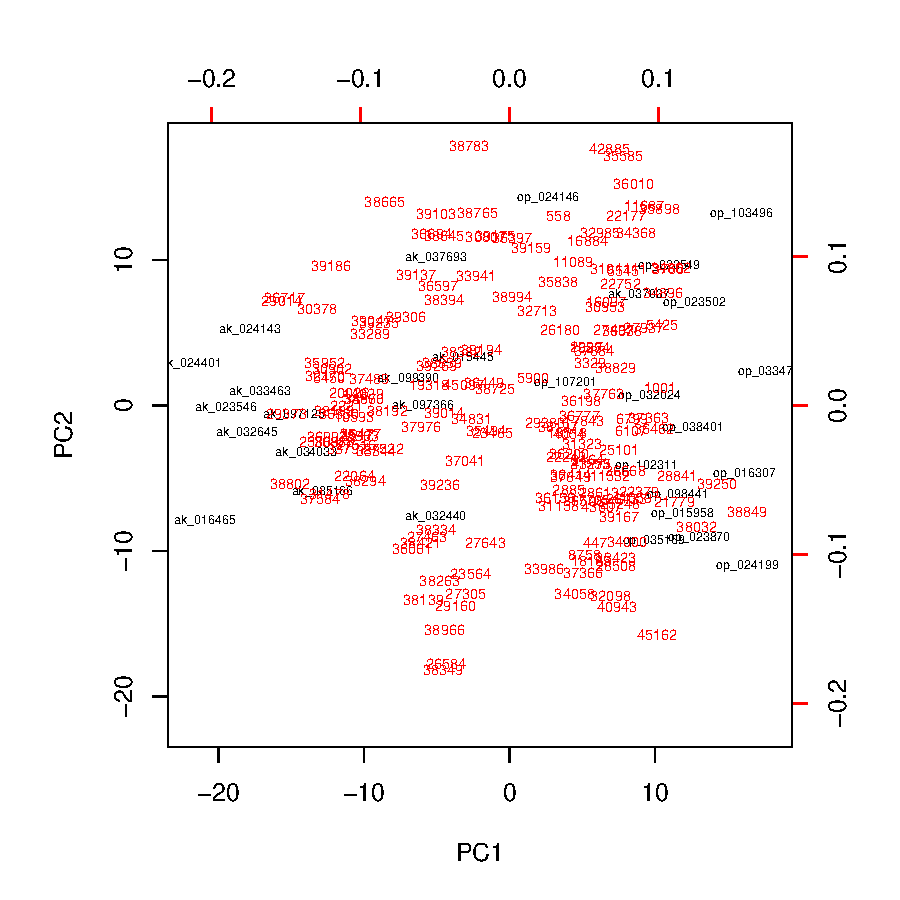
\includegraphics{CoDaSeq_vignette-003}
\end{center}
\end{figure}
\newpage

\subsection{Stripcharts}

\begin{figure}\label{strip chart}
\begin{center}
\begin{Schunk}
\begin{Sinput}
> # perform the singular value decomposition on clr transformed values
> conds <- c(rep("A", 15), rep("O", 15))
> f.x <- aldex.clr(f, conds)
\end{Sinput}
\begin{Soutput}
[1] "operating in serial mode"
[1] "Computing center with all features."
\end{Soutput}
\begin{Sinput}
> f.e <- aldex.effect(f.x, conds)
\end{Sinput}
\begin{Soutput}
[1] "operating in serial mode"
[1] "sanity check complete"
[1] "rab.all  complete"
[1] "rab.win  complete"
[1] "rab of samples complete"
[1] "within sample difference calculated"
[1] "between group difference calculated"
[1] "group summaries calculated"
[1] "effect size calculated"
[1] "summarizing output"
\end{Soutput}
\begin{Sinput}
> f.t <- aldex.ttest(f.x, conds)
> f.all <- data.frame(f.e,f.t)
> codaSeq.stripchart(aldex.out=f.all, group.table=hmpgenera, group.label="genus", 
+     p.cutoff=0.05, x.axis="effect")
\end{Sinput}
\end{Schunk}
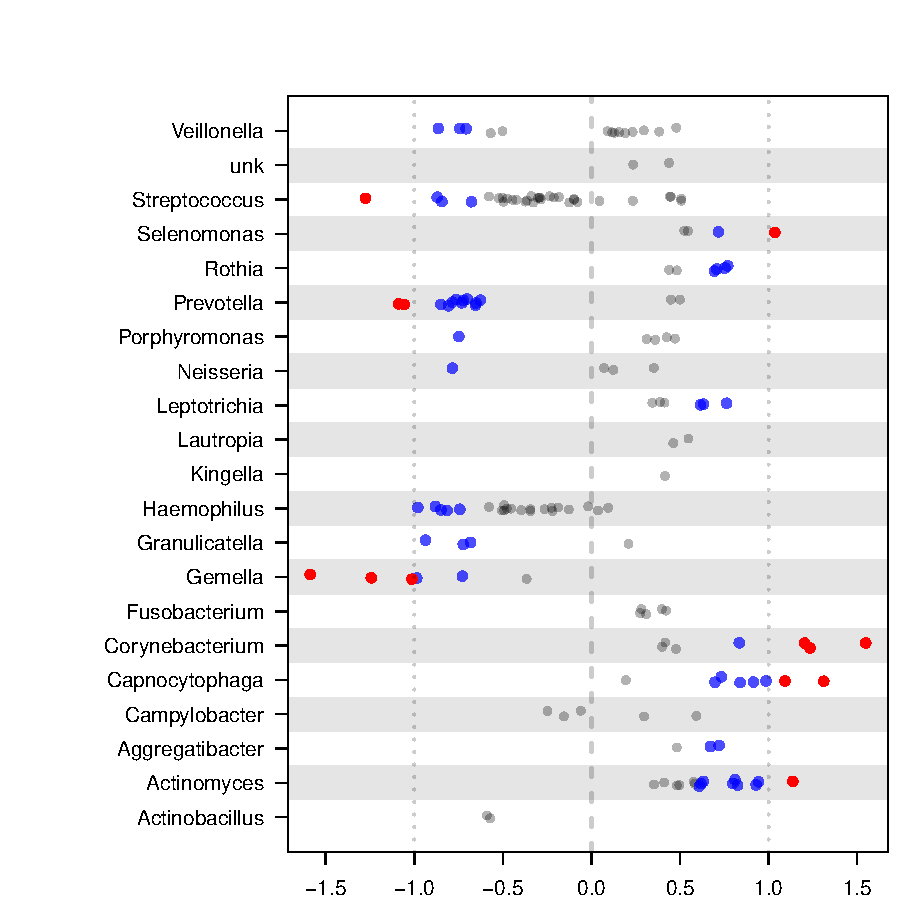
\includegraphics{CoDaSeq_vignette-004}
\end{center}
\end{figure}
 

\newpage

\subsection{Correcting for asymmetric datasets}
ALDEx2 now includes methods to centre the data properly when the dataset contains an asymmetry between the groups. An asymmetry can arise for many reasons: in RNA-seq it could arise because samples in one group contain a plasmid and the samples in the other group do not; in metagenomics or 16S rRNA gene sequencing it can arise when the samples in the two groups are taken from different environments; in a selex experiment it can arise because the two groups are under different selective constraints. The asymmetry can manifest either as a difference in sparsity (i.e., one group contains more 0 value features than the other) or as a systematic difference in abundance. When this occurs the geometric mean of each group can be markedly different, and thus an inherent skew in the dataset can occur that leads to false positive and false negative feature calls.

ALDEx2 now incorporates three approaches to deal with asymmetric datasets:

\begin{enumerate}
\item{\emph{all}: The default  is to calculate the geometric mean of all features. This is the approach used in previous versions of ALDEx2, and is the usual method for the compositional data analysis approach.}
\item{\emph{iqlr}: The first new approach is to identify those features that exhibit reproducible variance in the entire dataset. This is called the inter-quartile log-ratio or \emph{iqlr} approach. For this, a uniform prior of 0.5 is applied to the dataset, the clr transformation is applied, and the variance of each feature is calculated. Those features that have variance values that fall between the first and third quartiles of variance for all features are retained. When aldex.clr is called, the geometric mean abundance of only the retained features is calculated and used as  the denominator for log-ratio calculations. Modelling shows that this approach is effective in dealing with datasets with minor amounts of asymmetry, and begins to fail when more than 25\% of the features are asymmetric. The approach has the advantage it has little or no effect on symmetric datasets and so is a safe approach if the user is unsure if the data is mildly asymmetric.  }
\item{\emph{zero}: The second new approach is to identify those features that are non-zero in each group. In this approach the per-group non-zero features are used aldex.clr calculates the geometric mean in the clr transformation. This method is appropriate when the groups are very asymmetric, but the experimentalist must ask whether the comparison is valid in these extreme cases.}
\item{\emph{user}: The third new approach is to let the user define the set of `invariant' features. In the case of meta-rna-seq, it could be argued that the levels of housekeeping genes should be standard for all samples. In this case the user could define the row indices that correspond to the particular set of housekeeping genes to use as the standard. \emph{It is important that no row contain all 0 values for any feature when this method is used.} }
\end{enumerate}

 %%%
\newpage
\section{Contributors}
Andrew Fernandes wrote the original ALDEx code, and designed ALDEx2. Jean Macklaim found and squished a number of bugs, performed  testing, did much of the validation. Matt Links incorporated several ALDEx2 functions into a multicore environment. Adrianne Albert wrote the correlation and the one-way ANOVA modules. Ruth Grace Wong added function definitions and made the parallel code functional with BioConducter. Jia Rong Wu developed and implemented the alternate denominator method to correct for asymmetric datasets. Andrew Fernandes, Jean Macklaim and Ruth Grace Wong contributed to the Sum-FunctionsAitchison.R code. Greg Gloor is currently maintaining ALDEx2 and played roles in design and implementation.

\section{Version information}

\end{document}
